Magnetism with a spin at spin wave (pun totally intended).

\begin{parts}
	\part Standard derivation similar to Q5 2021.
	
	$B_\textnormal{mf}$ is the molecular mean field of the lattice -- this is the effective average magnetic field experienced by a spin as a result of the exchange interaction.
	
	Next we examine the Heisenberg exchange Hamiltonian for each spin in the magnetic structure from the question:
	\begin{align}
		\mathcal{H}_i &= \sum_{ij}\frac{J}{2} \, \mathbf{S}_i \cdot \mathbf{S}_j \notag \\
		&= 6 \times \frac{J}{2} \times \left(-S^2\right) \notag \\
		&= -3JS^2 \label{eqn:q4-heisenberg}
	\end{align}
	where the factor of $\diagfrac{1}{2}$ comes from the over-counting in unfolding the sum $\langle ij \rangle \rightarrow ij$.
	
	Equating \eqref{eqn:q4-heisenberg} with $g \mu_B B_\textnormal{mf} S_{i}$ then gives
	\begin{equation}
		B_\textnormal{mf} = -\frac{3JS}{g \mu_B}
		\label{eqn:q4-mean-field}
	\end{equation}
	
	Now recall magnetisation $M = \mu_\textnormal{total} / V$ where $\mu_\textnormal{total}$ is the total magnetic moment in a magnetic unit cell of volume $V$:
	\begin{align}
		M &= \frac{4 g \mu_B S}{\left(2a\right)^3} \notag \\
		&= \frac{g \mu_B S}{2a^3}
		\label{eqn:q4-magnetisation}
	\end{align}
	since each sublattice in the question is an FCC lattice with lattice parameter $2a$.
	
	Comparing \eqref{eqn:q4-mean-field} and \eqref{eqn:q4-magnetisation} then gives
	\begin{equation*}
		\lambda = \frac{6Ja^3}{\left(g \mu_B\right)^2}
	\end{equation*}
	
	We then substitute from left to right to get $T_\textnormal{N}$, noting that $M_s$ follows from \eqref{eqn:q4-magnetisation} and invoking the small $y$ approximation gives:
	\begin{align}
		M_\textnormal{A} &\approx \frac{g \mu_B S}{2a^3} \frac{S+1}{3S} y \notag \\
		&= \frac{g \mu_B S}{2a^3} \frac{S+1}{3S} \frac{g \mu_B S}{k_B T_\textnormal{N}} \left( \frac{6Ja^3}{\left(g \mu_B\right)^2} M_\textnormal{A} \right) \notag \\
		\Rightarrow T_\textnormal{N} &= \frac{JS\left(S+1\right)}{k_B}
		\label{eqn:q4-tn}
	\end{align}
	
	\newpage
	\part From the graph, we see that the maximum energy occurs at $\left(\frac{1}{2},\, \frac{1}{2},\, 0\right)$. This corresponds to $\gamma_\mathbf{k} = \left[-1-1+1\right]/3 = -\diagfrac{1}{3}$. Hence
	\begin{gather}
		E_\textnormal{max} = 6SJ \sqrt{1 - \frac{1}{9}} \notag \\
		J = \frac{E_\textnormal{max}}{4\sqrt{2}S} = \SI{0.566}{\milli\electronvolt}
		\label{eqn:q4-j}
	\end{gather}
	for $E_\textnormal{max} \approx \SI{8}{\milli\electronvolt}$, $S=\diagfrac{5}{2}$.
	
	Sketch of dispersion for path $\left( 0,\, 0,\, \frac{1}{2}\right) \rightarrow \left(0,\, 0,\, 0\right) \rightarrow \left(\frac{1}{2},\, \frac{1}{2},\, \frac{1}{2}\right)$ by tracing out the cosine term:
	\begin{gather*}
		\gamma_\mathbf{k} = 
		\begin{cases}
			\frac{1}{3} \textnormal{\hspace{1em}@}(0,\, 0,\, \frac{1}{2}) \\
			1 \textnormal{\hspace{1em}@}(0,\, 0,\, 0) \\
			-\frac{1}{3} \textnormal{\hspace{1em}@}(\frac{1}{2},\, \frac{1}{2},\, \frac{1}{2}) \\
			0 \textnormal{\hspace{1em}@}(\frac{1}{4},\, \frac{1}{4},\, \frac{1}{4})
		\end{cases}
	\end{gather*}
	\begin{figure}[H]
		\centering
		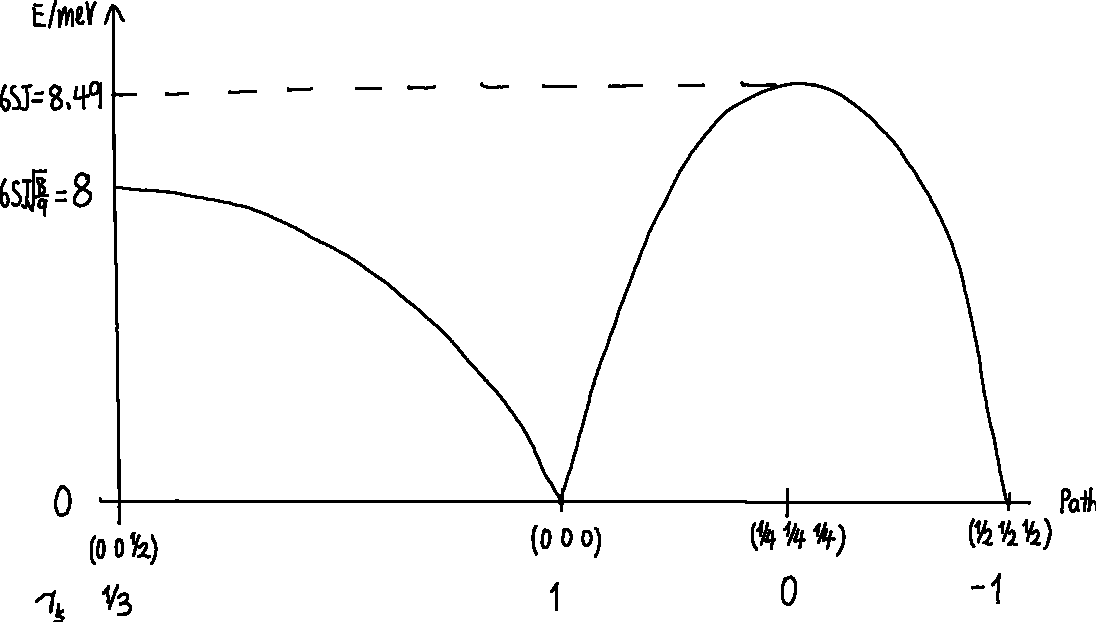
\includegraphics[width=.8\linewidth]{q4-dispersion}
	\end{figure}
	
	Gapless spin-wave spectrum suggests that we have a \textit{spontaneous symmetry breaking} and the universality class of the transition is \textit{3D Heisenberg}.
	
	Substituting \eqref{eqn:q4-j} into \eqref{eqn:q4-tn} gives $T_\textnormal{N} = \SI{57}{\kelvin}$.
	This is lower than the measured value $T_\textnormal{N}^\textnormal{exp} = \SI{83}{\kelvin}$ as the mean-field theory ignores fluctuations in the exchange interactions, which then lead to it underestimating the interaction energy.
	
	\part For small wavevector, we first rewrite $\gamma_\mathbf{k}$ as
	\begin{align*}
		\gamma_\mathbf{k} &= \frac{\cos(k_x a) + \cos(k_y a) + \cos(k_z a)}{3} \\
		&\approx \frac{(1-k_x^2 a^2 / 2) + (1-k_y^2 a^2 / 2) + (1-k_z^2 a^2 / 2)}{3} \\
		&= 1-\frac{|\mathbf{k}|^2 a^2}{6}
	\end{align*}
	
	Therefore the dispersion may be approximated as
	\begin{align*}
		\hbar\omega_\mathbf{k} &= 6SJ \sqrt{1 - \gamma_\mathbf{k}^2} \\
		&\approx 6SJ \sqrt{1 - \left(1 - \frac{|\mathbf{k}|^2 a^2}{3}\right)} \textnormal{\hspace{1em}ignoring higher order terms} \\
		&= 6SJ \frac{|\mathbf{k}| a}{\sqrt{3}} \\
		\Rightarrow \omega_\mathbf{k} &\approx \underbracket{\frac{6SJa}{\sqrt{3}\hbar}}_{c} \left|\mathbf{k}\right|
	\end{align*}
	
	Energy of an ensemble of spin waves, with $n_\textnormal{B} = [\exp(E/k_\textnormal{B} T) - 1]^{-1}$ being the Bose occupation factor:
	\begin{equation*}
		E = \int_{0}^{\infty} g(E) \, n_\textnormal{B} \, E \, \mathrm{d}E
	\end{equation*}
	
	Assuming isotropy, we then have the following d.o.s. due to the linear dispersion:
	\begin{align*}
		g(k)\, \mathrm{d}k &= \frac{2}{(2\pi)^3}\, 4\pi k^2\, \mathrm{d}k \\
		&= \frac{2}{(2\pi)^3}\, 4\pi \left(\frac{E}{\hbar c}\right)^2 \frac{\mathrm{d}E}{\hbar c} \\
		&= \frac{1}{\pi^2 \hbar^3 c^3}\, E^2\, \mathrm{d}E \\
		&= g(E)\, \mathrm{d}E
	\end{align*}
	
	Thus the total energy is
	\begin{align}
		E &= \int_{0}^{\infty} \mathrm{d}E\, \frac{1}{\pi^2 \hbar^3 c^3} E^2 \, \frac{1}{\exp(E/k_\textnormal{B} T) - 1} \, E \notag \\
		&= \frac{1}{\pi^2 \hbar^3 c^3} \int_{0}^{\infty} \frac{E^3}{\exp(E/k_\textnormal{B} T) - 1}\, \mathrm{d}E \notag \\
		&= \frac{1}{\pi^2 \hbar^3 c^3} \int_{0}^{\infty} \left(k_\textnormal{B} T\right)^4 \frac{x^3}{\exp(x) - 1}\, \mathrm{d}x \textnormal{\hspace{1em}where $x=E/k_B T$} \notag \\
		&= \frac{k_\textnormal{B}^4}{\pi^2 \hbar^3 c^3}\, T^4
		\label{eqn:q4-spin-wave-energy}
	\end{align}

	Differentiating \eqref{eqn:q4-spin-wave-energy} w.r.t. $T$ yields the heat capacity per volume due to spin waves in the low temperature limit:
	\begin{align*}
		C_m &= \left( \frac{\partial E}{\partial T} \right)_{V} \\
		&= \frac{4k_\textnormal{B}^4}{\pi^2 \hbar^3 c^3}\, T^3
	\end{align*}
\end{parts}